En este capítulo se detallan las baterías de pruebas a las que se ha sometido
\textbf{SiteUp}, ya sean de carácter manual o automatizadas mediante software
específico.

\section{Estrategia}

La estrategia de pruebas seguida en SiteUp es híbrida. Por un lado, se cuenta
con una batería de pruebas automatizada, basadas en el motor de pruebas que
incluye el framework de desarrollo, que verifican las funcionaldiades más
críticas del sistema.

Por otro lado, se cuenta con pruebas manuales realizadas de forma periódica. A
corto plazo y de forma frecuente se revisaban las funcionalidades más inmediatas
de las aplicaciones. A largo plazo, se han dado de alta numerosos chequeos y se
han verificado a lo largo del tiempo.

\section{Entorno de pruebas}

Para las pruebas automáticas, el entorno de pruebas es una copia virtual del
entorno de producción real, creado automáticamente por el software de testeo, de
forma que no se modifiquen los valiosos datos de la base de datos de
producción. En cada ejecución de los tests se crea una base de datos y un
entorno nuevos, vacíos, en los que se llevan a cabo las pruebas.

Para las pruebas manuales, dado que se realizan directamente sobre el sistema en
producción, el entorno coincide con lo dispuesto en la
sección~\ref{subsec:entorno-produccion}.

\section{Roles}

Se presentan dos roles principales necesarios para la ejecución de las pruebas.

\subsection{Desarrollador principal}

En primer lugar, el desarrollador del producto es el principal probador del
software. Por un lado, es el encargado del desarrollo y ejecución de las
baterías de pruebas automatizadas, teniendo la obligación de interpretar los
resultados y actuando en consecuencia.

Por otro lado, también ha de probar el producto manualmente como un usuario más,
sobre todo a tenor de lo expuesto en la sección~\ref{sec:situacion-actual}, en
la que se refleja que la motivación principal del proyecto es una necesidad
personal del desarrollador.

\subsection{Probadores externos}

Además del desarrollador principal fue conveniente contar con la ayuda de varios
probadores externos que dieran su punto de vista sobre el software, como
usuarios. Así, realizaron pruebas de caracter manual a corto plazo, opinando
sobre la interfaz de usuario, la usabilidad y la accesibilidad del proyecto, así
como a largo plazo, dando de alta diversos chequeos y probando su funcionalidad.

En todas las etapas, el desarrollador obtenía feedback de los probadores,
integrando en la medida de lo posible los consejos y apreciaciones que se obtenían.


\section{Pruebas funcionales}

Las pruebas funcionales engloban las pruebas que tratan de comprobar el correcto
cumplimiento de los requisitos funcionales, de forma directa (verificando su
cumplimiento de forma directa) como de forma indirecta a varios niveles
(verificando que las dependencias de las que pende la funcionalidad funcionen
correctamente).

En primer lugar, se usaron \textbf{pruebas unitarias}, que tuvieron por objetivo
localizar errores en los elementos software antes de ser integrados con el resto
de elementos del sistema.

En SiteUp, el grueso de las pruebas unitarias se centró principalmente en el
módulo de chequeo, organizado dentro de la aplicación
\texttt{siteup\_checker}. Los diversos casos de test comprobaron de forma
individual que los procedimientos que llevan a cabo los chequeos devuelvan el
resultado correcto, asegurando la ausencia de falsos positivos y resultados
erróneos.

Por ejemplo, para la verificación del procedimiento de \textbf{chequeo HTTP} se
hizo uso del sitio web \textbf{HttpBin}~\cite{httpbin}, una web especialmente
pensada para facilitar el testeo de conexiones HTTP. 

La implementación de las pruebas se ha hecho utilizando las capacidades de
testing que provee el framework Django. Las pruebas unitarias se lanzan a través
de la línea de comandos, indicando el módulo de test unitario que se quiere
comprobar, por ejemplo:

\begin{bashcode}
$ python manage.py test siteup_checker.tests.test_http
Creating test database for alias 'default'...

(output omitted)

----------------------------------------------------------------------
Ran 7 tests in 2.506s

OK
Destroying test database for alias 'default'...
\end{bashcode} 

Tras la ejecución de los tests se muestra una lista de aquellos que han fallado,
ya sea por no haberse cumplido los asertos definidos o por otro error no
controlado. 

Por otro lado, Las \textbf{pruebas de integración} tuvieron por objetivo
localizar errores en módulos completos, analizando la interacción entre varios
artefactos software.

Como ejemplo, tras realizar las pruebas unitarias en los módulos de chequeo, se
pasó a hacer pruebas de integración entre los procedimientos de chequeo y las
instancias de los modelos de chequeo dadas de alta por los usuarios, de forma
que se asegurase que la creación de un chequeo por parte de un usuario era
reflejada en la base de datos y daba lugar a la correcta ejecución del
procedimento de chequeo. La forma de implementar estas pruebas fue, de nuevo,
utilizando el framework de testeo de Django.

\subsection{Pruebas de sistema}

Las pruebas de sistema, que buscan asegurar que el sistema cumple con todos los
requisitos establecidos, se desarrollaron de forma continua a medida que iba
avanzando el proyecto. 

En cada iteración, las pruebas se llevaron a cabo utilizando un entorno virtual
y el servidor de pruebas que integra el propio framework Django, y se utilizó
software de \textit{throttling} de red para simular condiciones de red adversas
que se asemejasen a las condiciones reales.

\subsection{Pruebas de aceptación}

Para verificar que el producto estaba listo para el paso a producción se hizo un
despliegue en un servidor real, ubicado en Alemania, y se dio de alta una decena
de chequeos de todos los tipos. El servidor ha permanecido online desde mediados
del mes de febrero hasta la fecha.

En este tiempo, además de recibir las actualizaciones del software a medida que
el desarrollo avanzaba, el proyecto ha detectado de forma eficiente las caídas
en el servicio de los chequeos dados de alta, notificando de manera correcta
tanto por correo electrónico como a través de la aplicación de Android.

En particular se puede poner de ejemplo la web oficial de la Universidad de
Cádiz, que se ha utilizado como objetivo de los chequeos. En el tiempo que ha
estado el chequeo activo se han detectado caídas en la web unas 15 veces, la
última el 16 de abril de 2014, día en el que durante la mañana la web ha pasado
a estar inaccesible más de 7 veces durante periodos de entre 10 y 30 minutos.


\section{Pruebas no funcionales}

Las pruebas no funcionales buscan verificar aspectos del proyecto más allá de su
funcionalidad, tales como la seguridad del sitio, su estabilidad, la
accesibilidad, etcétera.

\subsection{Pruebas de seguridad}

Las pruebas de seguridad se centraron en verificar que la información de los
usuarios y las áreas privadas del sitio web son seguras. Entre las pruebas que
se realizaron se encuentran las siguientes:

\begin{itemize}
\item Se intentó acceder a URLs de la plataforma web sin haber iniciado sesión,
  para comprobar que el control de usuarios es correcto. Por ejemplo, intentando
  acceder sin haber hecho login a la URL

\begin{verbatim}
http://siteup.josetomastocino.com/dashboard
\end{verbatim}

  La plataforma web actuó correctamente en estos casos, redirigiendo al usuario
  a la pantalla de login.

\item Se intentó obtener información de chequeos de otros usuarios, para ver si
  había filtración de datos, cambiando manualmente los identificadores
  enviados. Por ejemplo, la siguiente URL

\begin{verbatim}
http://siteup.josetomastocino.com/checks/pingcheck/6/
\end{verbatim}

  pertenece a la página de detalle del \texttt{PingCheck} con identificador 6,
  perteneciente a un usuario. Si intentamos acceder a esa URL con otro usuario,
  la plataforma web detecta este intento y no muestra el recurso, sino que
  muestra un error 404.

\item Se intentaron llevar a cabo varias inyecciones sql~\cite{inyeccion_sql},
  consistentes en escribir código SQL malicioso en los formularios de la
  plataforma web para ver si llegaban a ejecutarse en la base de datos. La
  plataforma web a través de los sistemas de saneado de formularios con los que
  cuenta consiguió que estos intentos no tuvieran efecto.
\end{itemize}

\subsection{Pruebas de fiabilidad}

Se comprobó satisfactoriamente el cumplimiento del requisito no funcional
\textit{NRQ-3}, que impone que los retrasos en el lanzamiento de chequeos no
pueden superar el 200\% del tiempo entre chequeos.

Para ello, se añadió una carga importante de chequeos en el sistema y se
monitorizaron las operaciones de Celery. En todos los casos la cola de prioridad
del sistema de tareas asíncronas permitió que los chequeos se ejecutaran dentro
de su \textit{slot} de tiempo adecuado, nunca superando la limitación
previamente dispuesta.

\subsection{Pruebas de accesibilidad}

El requisito no funcional \textit{NRQ-4} dictaminaba que \textit{la plataforma
  web deberá ser accesible desde cualquier clase de dispositivo móvil con acceso
  a internet}. Para verificar su cumplimiento se probó la plataforma web en los
siguientes dispositivos, siendo satisfactoria la navegación en todos ellos:

\begin{itemize}
\item Ordenador de mesa con navegadores Google Chrome, Firefox y IE 11, y
  resoluciones hasta 1024x768.
\item Tablet Google Nexus 7 de primera generación.
\item Samsung Galaxy Nexus.
\item Jiayu G2.
\item Apple iPad 2
\end{itemize}

Se presentan en las figuras \ref{fig:captura_ipad}, \ref{fig:captura_jiayu} y
\ref{fig:captura_galaxy} algunas capturas de pantalla de la web en diversos
dispositivos.

\begin{figure}[hbtp]
  \centering
  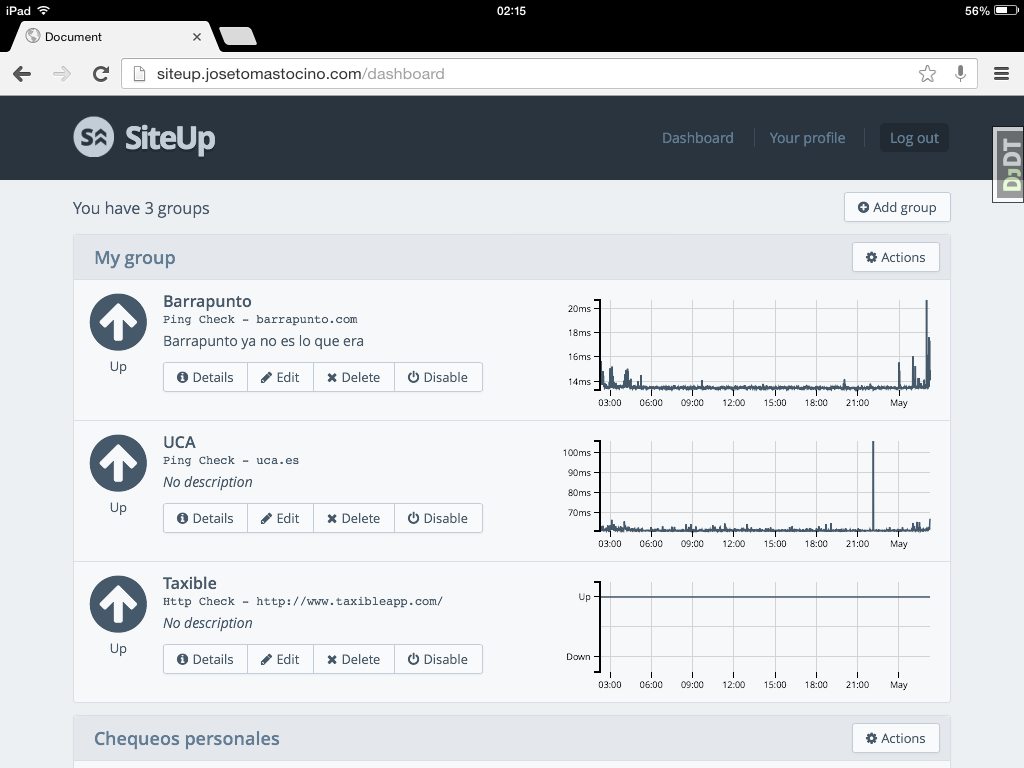
\includegraphics[width=\textwidth]{7_pruebas/captura_ipad}
  \caption{Plataforma web vista mediante un Apple iPad 2}
  \label{fig:captura_ipad}
\end{figure}


\begin{figure}[hbtp]
  \centering
  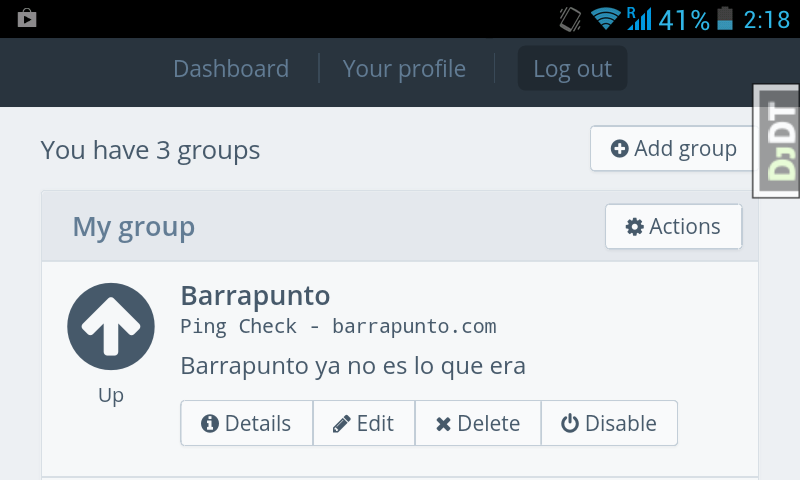
\includegraphics[width=0.7\textwidth]{7_pruebas/captura_jiayu}
  \caption{Plataforma web vista mediante un Jiayu G2 (orientación horizontal)}
  \label{fig:captura_jiayu}
\end{figure}

\begin{figure}[hbtp]
  \centering
  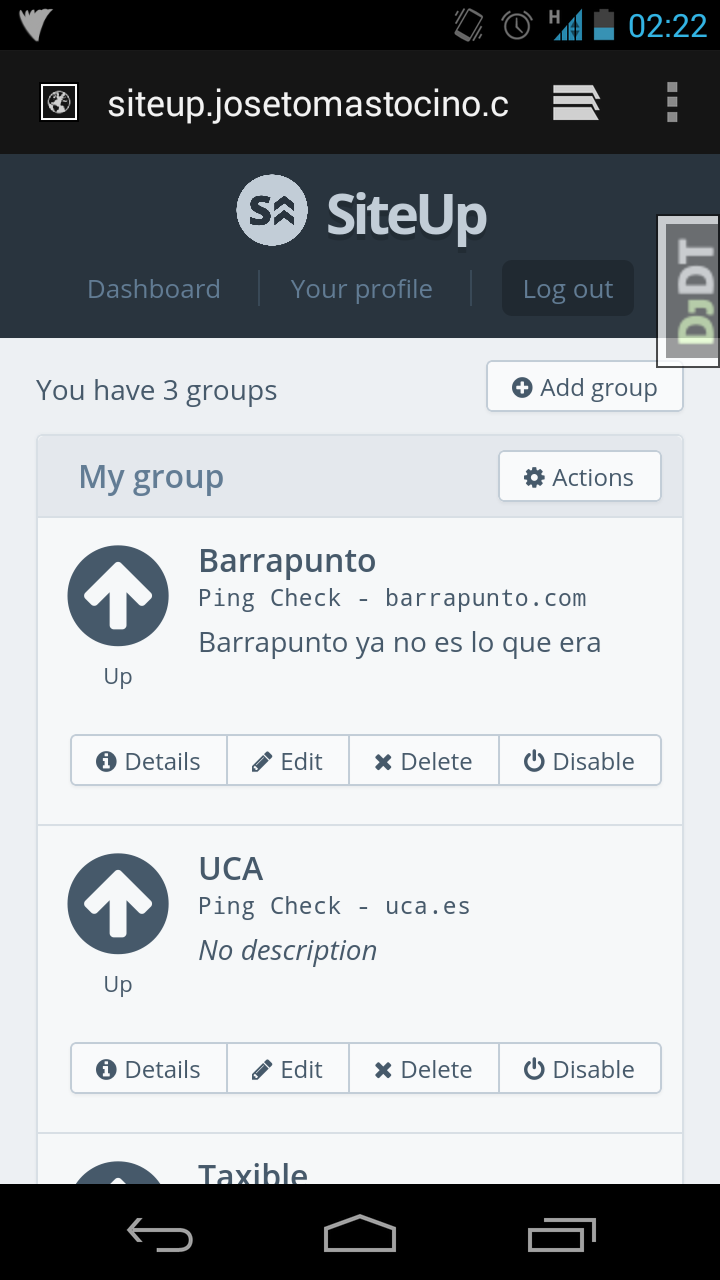
\includegraphics[width=0.7\textwidth]{7_pruebas/captura_galaxy}
  \caption{Plataforma web vista mediante un Galaxy Nexus }
  \label{fig:captura_galaxy}
\end{figure}

\subsection{Verificación de la calidad del código}

En la medida de lo posible se ha seguido la guía de estilo oficial de Python,
expuesta en el documento oficial PEP8~\cite{pep8} por el propio creador del
lenguaje, Guido van Rossum. Para reforzar el seguimiento de estas buenas
prácticas de código se ha hecho uso de herramientas de verificación automática,
que comprueban que el código se ajuste a las convenciones de nombrado, sintaxis
y otras recomendaciones presentes en el citado documento.


% \section{Implementación de pruebas}

% Como se ha comentado, 

%%% Local Variables: 
%%% mode: latex
%%% TeX-master: "../memoria"
%%% End: 
